\documentclass[11pt]{article}
\usepackage{graphicx}
\usepackage[export]{adjustbox}
\usepackage{float}
\usepackage{listings}
\usepackage{amsmath}
\usepackage{color}
\definecolor{lightgray}{gray}{0.9}
\title{EE302 Homework 3}
\date{2018\\ March}
\author{Nail Tosun - 2094563 -Section 5\\ Electric and Electronic Engineering Departmant, METU}
\begin{document}
\maketitle


\subsection*{4}
\subsubsection*{a)}

\lstset{
    showstringspaces=false,
    basicstyle=\ttfamily,
    keywordstyle=\color{blue},
    commentstyle=\color[grey]{0.6},
    stringstyle=\color[RGB]{255,150,75}
}

\newcommand{\inlinecode}[2]{\colorbox{lightgray}{\lstinline[language=#1]$#2$}}

\inlinecode{java}{
p1 = [1 20 10 400];}

\inlinecode{java}{
p2 = [1 3 2 6 3 1];}

\inlinecode{java}{
p3 = [1 -1 2 -4 -8];}

\inlinecode{java}{
p4 = [1 2 16 32 100 200];}

\inlinecode{java}{
roots1 = roots(p1);}

\inlinecode{java}{
roots2 = roots(p2);}

\inlinecode{java}{
roots3 = roots(p3);}

\inlinecode{java}{
roots4 = roots(p4);}
\vspace{5mm} %5mm vertical space

Results are (in 2 significant digit);
polynomial 1 has roots at 

$\lambda_1= -20,47 + 0,00i$

$\lambda_2= 0,23 + 4,41i$

$\lambda_3= 0,23 - 4,41i$

I expect two positive pole from routh-hurwitz test. Result make sense.
\vspace{5mm}

polynomial 2 has roots at

$\lambda_1=-2,91$

$\lambda_2=0,23 + 1,33i$

$\lambda_3=0,23 - 1,33i$

$\lambda_4=-0,28 + 0,34i$

$\lambda_5=-0,28 - 0,34i$

From Routh-Hurwitz test i expect 2 positive pole. Matlab result consistent.
\vspace{5mm}

polynomial 3 has roots at

$\lambda_1=2.00$

$\lambda_2=2.00i$

$\lambda_3=-2.00i$

$\lambda_4=-1.00$

From Routh-Hurwitz test i expect two poles on jw axis and one pole at RHP. Matlab results make sense.
\vspace{5mm}

polynomial 4 has roots at

$\lambda_1=1,00 + 3,00i$

$\lambda_2=1,00 - 3,00i$

$\lambda_3=-1,00 + 3,00i$

$\lambda_4=-1,00 - 3,00i$

$\lambda_5=-2,00$

From Routh-Hurwitz test i expect two RHP poles with quadrantal pair at LHP. Matlab result are same.
\begin{figure}[H]
  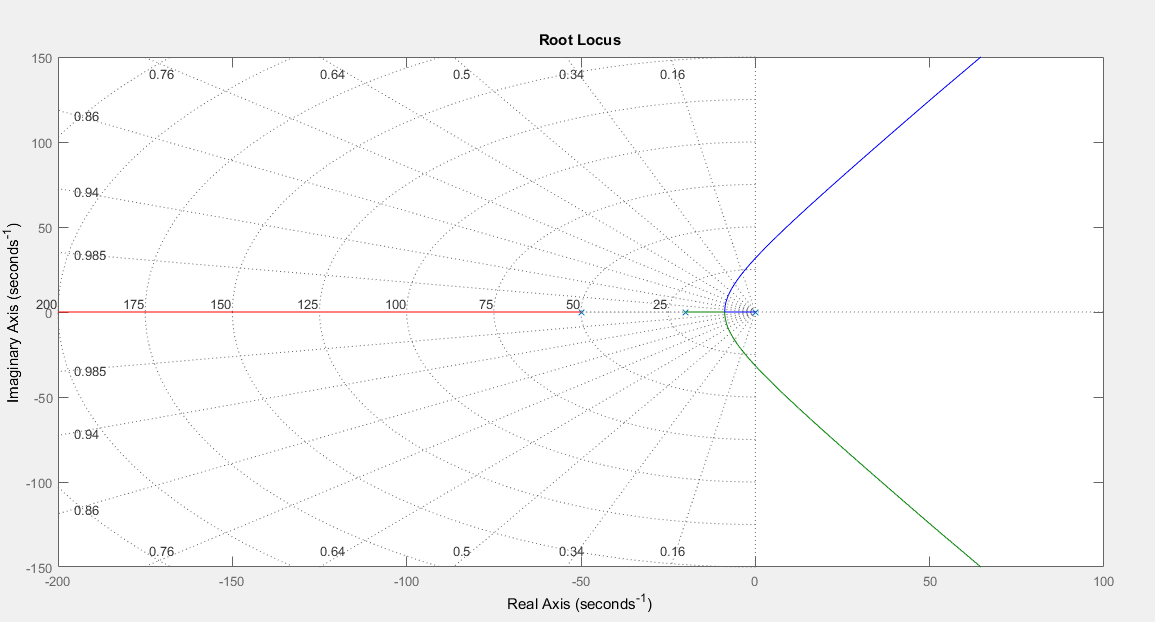
\includegraphics[scale=0.7, center]{3a}
  \caption{3a}
  \label{fig:zero}
\end{figure}
\begin{figure}[H]
  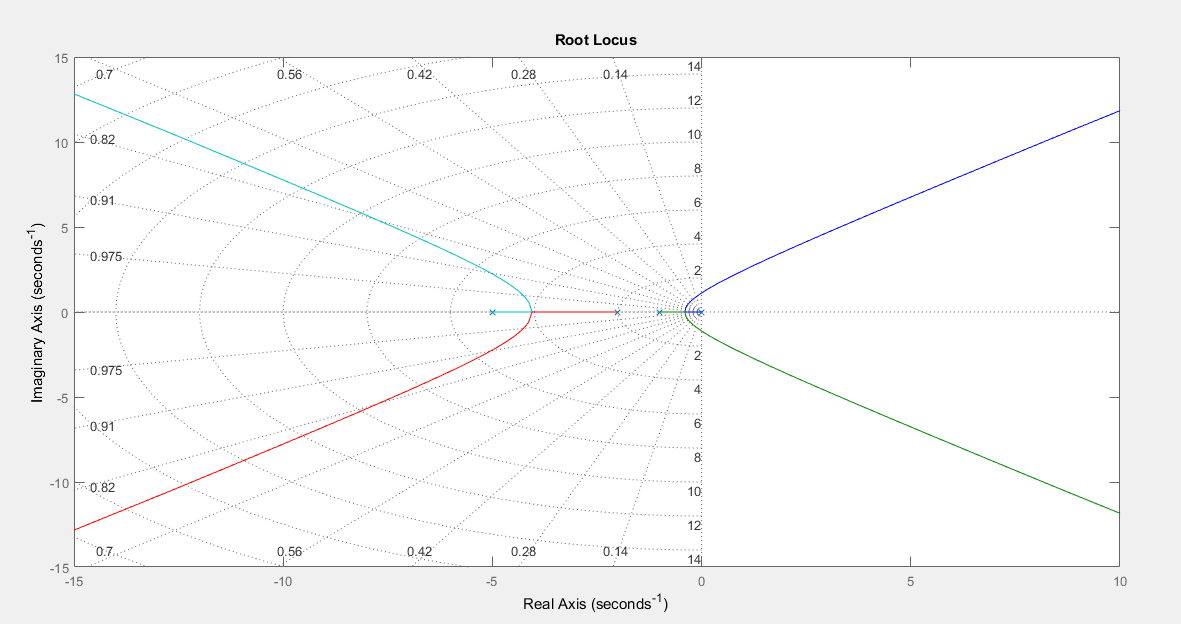
\includegraphics[scale=0.7, center]{3b}
  \caption{3b}
  \label{fig:zero}
\end{figure}
\begin{figure}[H]
  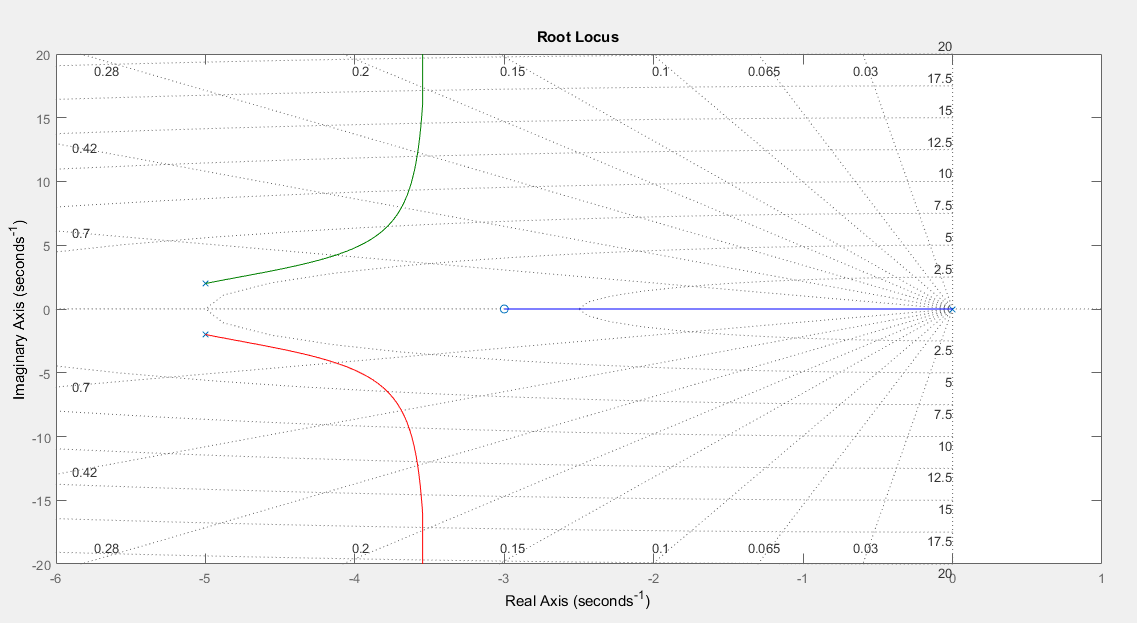
\includegraphics[scale=0.7, center]{3c}
  \caption{3c}
  \label{fig:zero}
\end{figure}
\begin{figure}[H]
  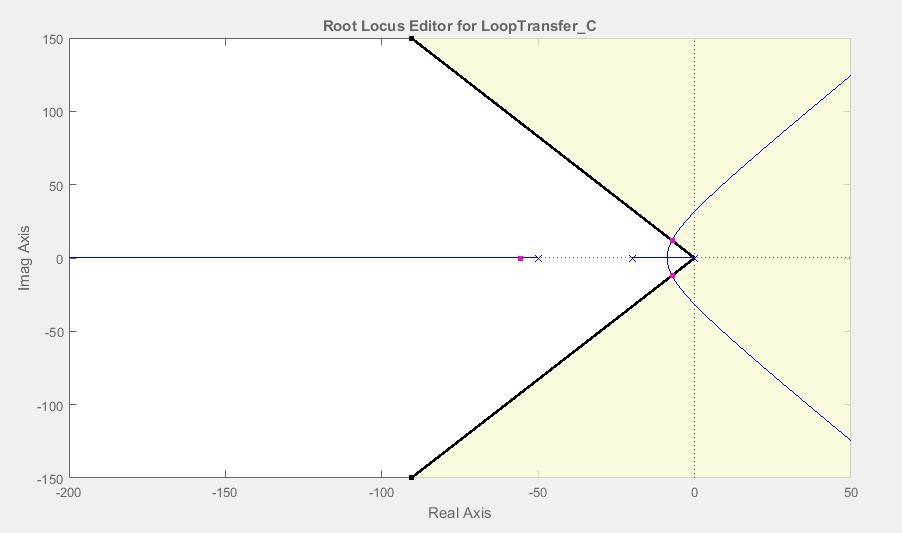
\includegraphics[scale=0.7, center]{4}
  \caption{root locus}
  \label{fig:zero}
\end{figure}
\begin{figure}[H]
  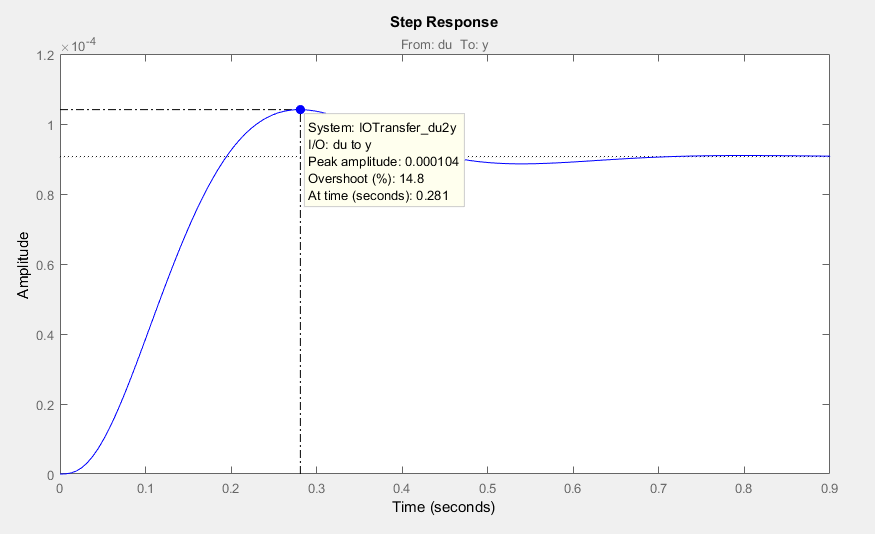
\includegraphics[scale=0.7, center]{4b}
  \caption{step response}
  \label{fig:zero}
\end{figure}
\end{document}